\subsection{Lorenz}

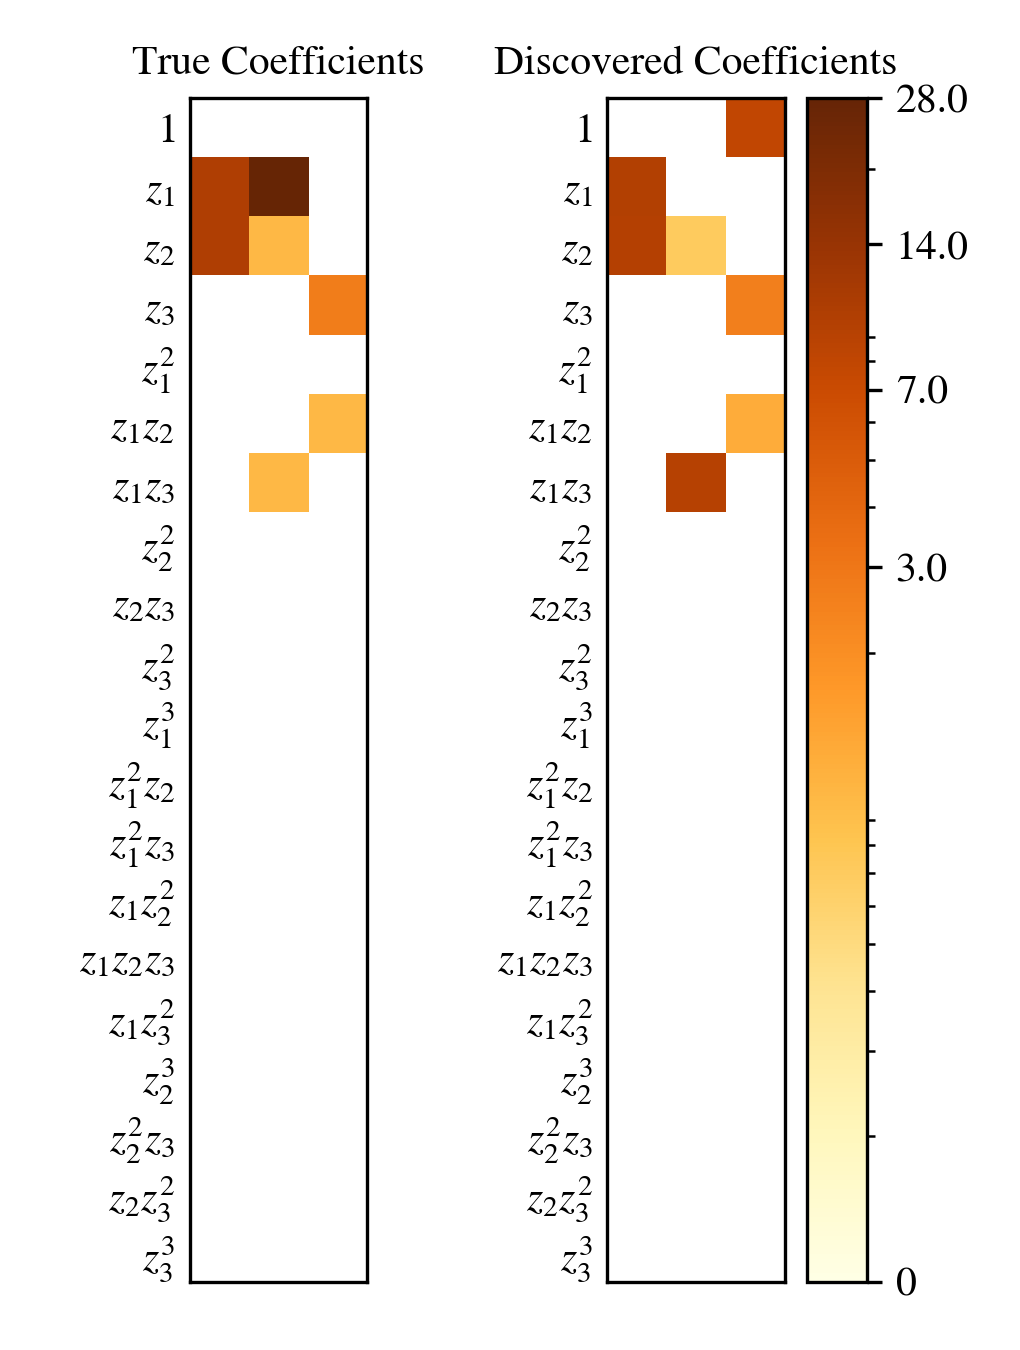
\includegraphics[width=0.48\textwidth]{project_2/images/xi_plot_lorenz.png}
\label{fig:xi_plot_lorenz}

\subsection{Pendulum}


\begin{figure}[htbp]
    \centering
    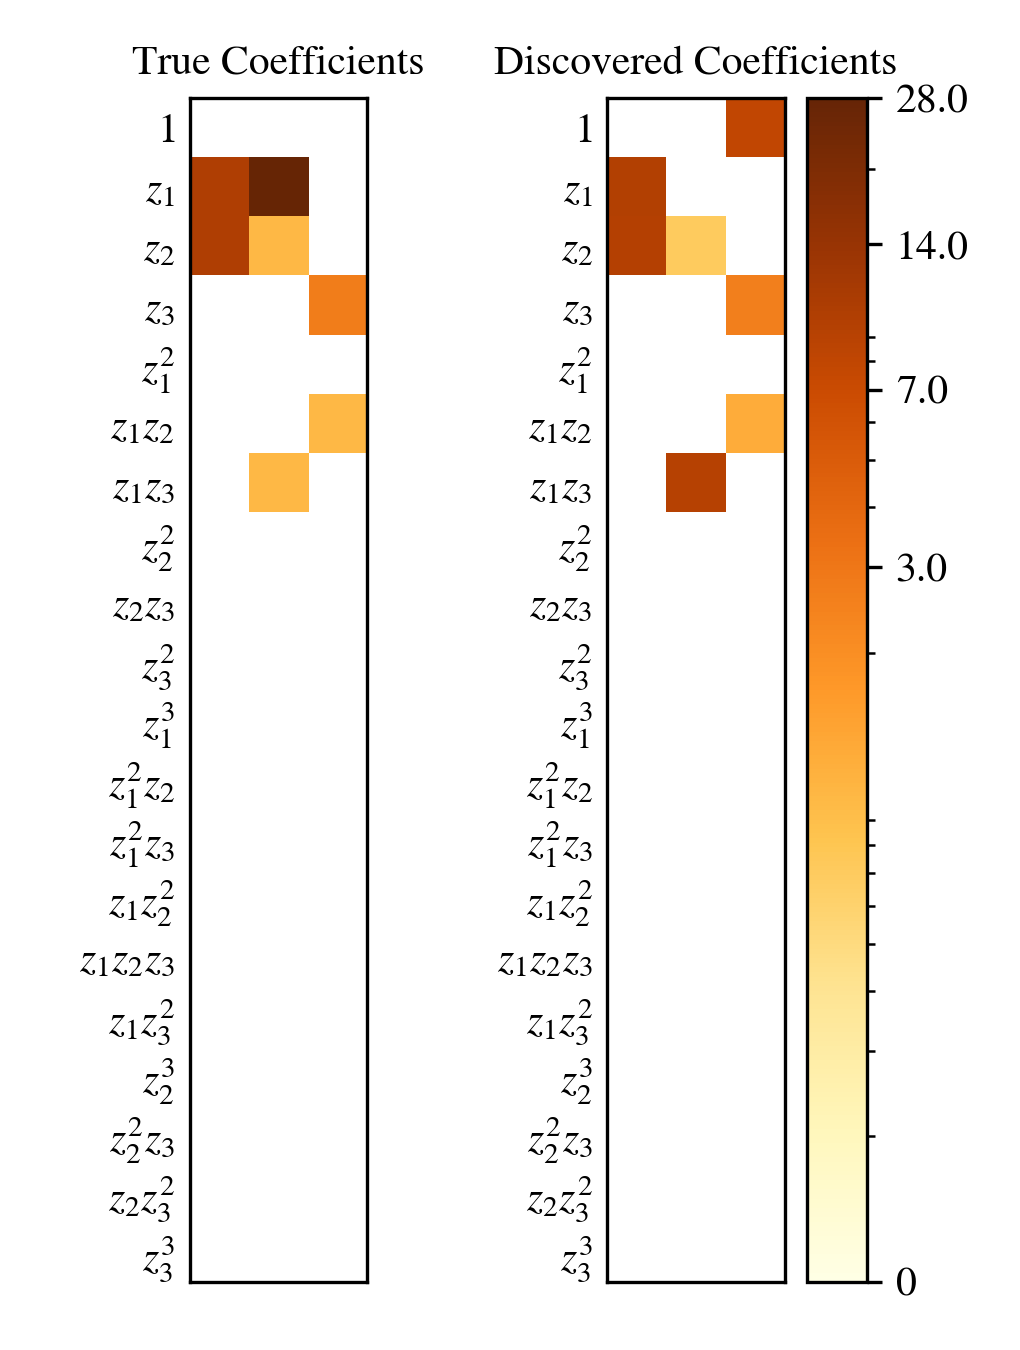
\includegraphics[width=0.48\textwidth]{project_2/images/xi_plot_lorenz.png}
    %\caption{}
    \label{fig:xi_plot_lorenz}
\end{figure}

For the pendulum simulation we trained five models of which three converged to one coefficient and two converged to the right coefficient.

The correct models accurately identified the dynamics governing the pendulum's motion. The discovered coefficients highlight that the model found the single nonlinear term $\sin (z_1)$, which is what gives the pendulum its periodic nature. All other terms have zero coefficients, correctly indicating that they do not contribute to the system dynamics.